\chapter{Path selection} \label{chap:steiner}

%\section{Subproblems}

Our approach to a better heuristic is driven by the concept of location graph and using the same for construction of low latency tours of the MULEs in data collection phase. The two critical subproblems encountered in this context are: 
(i) Euclidean Minimum Stiener Tree (EMST), and (ii)  Euclidean Travelling Saleman Problem (ETSP). Both the problems have already been introduced
in chapter 2. We will briefly restate these here for
sake of completeness and convenience in description of our heuristic.

%%%%%%%%%%%%%%%%%%%%%%%%%%%%%%%%%%%%%%%%%%%%%
\begin{definition}[Euclidean Travelling Salesman Problem]
Given a set of n 2D points in a plane find a minimum cost tour of all
the points, visiting every point exactly once.
\end{definition}
We use Christofides algorithm~\cite{christofides} as the approximation heuristic for computing TSP route of a set of points.

\begin{definition}[Euclidean minimum Steiner Tree problem]
Given a set $P$ of points in a 2-D plane as input, the output is a network of line segements connecting all of the points in $S$, with the smallest total (Euclidean) length.
\end{definition}
The line segments making the Steiner Tree need just be incident on the points in $S$. This implies that the algorithm is free to use additional points from the plane, if necessary, to produce the smallest total length network. The additional points are called {\em Steiner Points}.
%%%%%%%%%%%%%%%%%%%%%%%%%%%%%%%%%%%%%%%%%%%%%%%%%%%%%%%%%%%

The location nodes (the nodes in location graph) computed earlier, form the set $P$, and the EMST is generated using the set $P$, and is called the location graph $T$. The pseudo code for the heuristic which appear later in section ~\ref{sec:heuristicAlgo} uses the EMST as input. The choice of EMST as data structure over MST is guided by the fact that the weight (weight here means total of lengths of all the edges in a graph) of EMST is always atmost the weight of the MST, and we use the weight of a tree as an approximation of the weight of the TSP tour of its vertices.

The TSP time unit is the time taken by a MULE to visit all points on EMST. The cost of ETSP on a set is atmost twice the cost of the EMST on it. Therefore, it should be reasonable to use the Steiner tree traversal as a guide for partitioning. Furthermore, in the case where the field also includes obstacles, Steiner trees lend themselves naturally to cover all the points due the properties of Steiner points~\cite{oaest99} as explained in section~\ref{sec:steinerPoint} of chapter~2. Though we plan not to cover the obstacle avoidance case, we briefly sketch the underlying ideas in Chapter~\ref{chap:concl}. For computing Steiner tress, we use the exact solution finder software GeoSteiner~\cite{geosteiner1}~\cite{geosteiner2}~\cite{geosteiner3}. 


\begin{figure}[H]
\centering
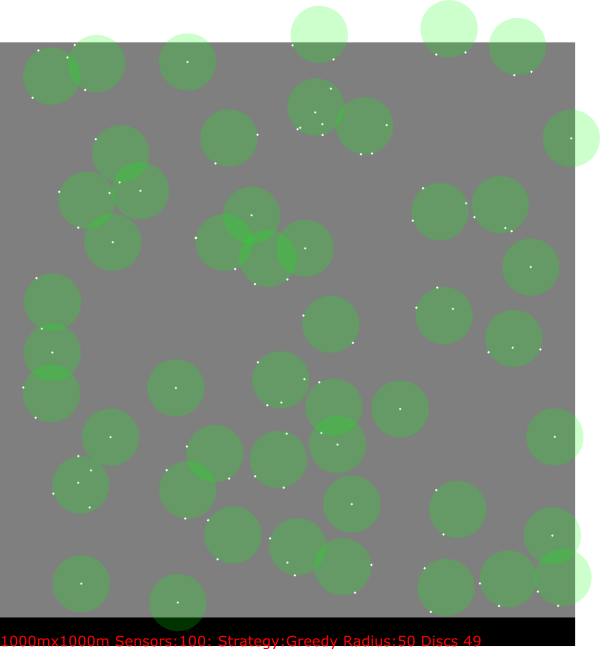
\includegraphics[width=6cm]{figures/disc100.png}
\caption{50m radius disc cover of 100 sensors in 1000x1000 field} \label{fig:disc100}
\medskip
\small
The white dots are sensor positions
\end{figure}

\begin{figure}[H]
\centering
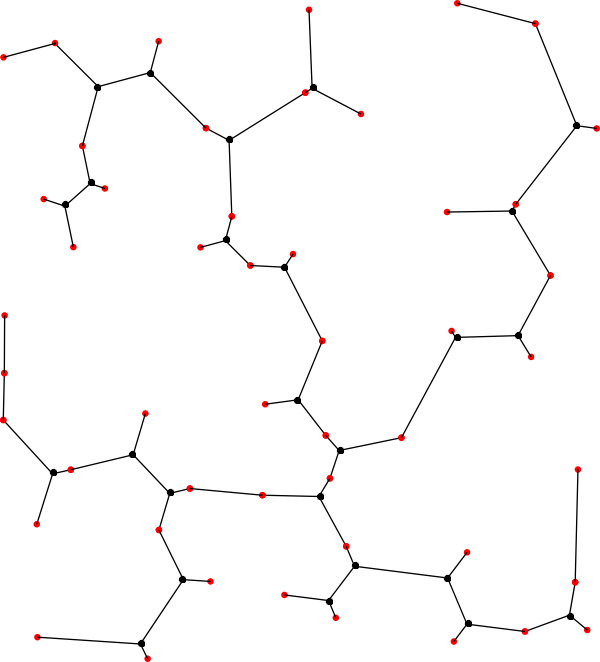
\includegraphics[width=6cm]{figures/steiner100.png}
\caption{The Steiner tree of disc centers of figure \ref{fig:disc100}}
\medskip
\small
The black dots are Steiner points and the red dots are disc centers
\end{figure}


\section{Path Selection Heuristic}

%\subsection{Aim}
The aim of path selection heuristic is to find a minimum partitioning of
the set of location nodes of a location graph by addition of 
extra Steiner points such that following conditions are satisfied.

\begin{itemize}
\item Each of the subsets has a TSP tour length (in units of time) less than a per-specified value $L$, and for any two sets $S_{i}$ and $S_{j}$, $S_{i} \cap S_{j} \le 1$.
\item Let $V$ be the set of all subsets $S_{i}$. Let $E$ be the set of pairs of subsets $(S_{i},S_{j})$ such that $S_{i} \cap S_{j} = 1$. Then the graph $G(V,E)$ should be a connected graph.
\end{itemize}

It assumed that the time a MULE spends in a network while collecting data
consists of three main components: (i) travelling from one location node to another $t_{TSP}$ (ii) Talking to sensors belonging to a location node $t_{LS}$, called MULE's pause time, at a location node (iii) Talking to other MULEs/Base station $t_{MBS}$.

We assume that MULE to MULE data transfer times are shorterdue to two reasons, namely, (i) MULEs may use data aggregation while sending data to fellow a MULE or BS, and (ii) MULEs being relative expensive and more robust than sensor node, typically have higher bandwidth for inter MULE data transfer. This is the reason, we ignore the contribution of $t_{MBS}$. The component $t_{LS}$ for each location node can be given as an input (observed before running the heuristic, by simply sending one MULE on a tour of all the location nodes in the field to measure and record such times beforehand), or computed using sensor parameters, such as: Sensor data throughput ($SDT$, effective data rate, after taking into account the overhead introduced due to protocol headers) and Sensor data sampling rate ($SSR$, data sampling rate of the sensor, the speed of data acquisition of the sensor from its environment in bytes/sec).


\subsection{Heuristic}

The overall strategy is to create an EMST of the location nodes and then divide this tree into subgraphs, using the tree edges as the guide. Each subgraph's set of nodes will be covered by one MULE (henceforth, this set of nodes will be called a subtour). The term "weight" is equivalent to "time interval" in this algorithm, and is measured in seconds. An edge of the tree is said to have weight equal to its length divided by the speed of the MULE (time taken by the MULE to cover that edge). The weight of a location node is equal to the time a MULE has to wait there for data collection (called pause time). It depends on the latency bound and the number of sensor nodes covered by that location node. Steiner points have zero weight. The weight of the TSP tour of a set of nodes is equal to the smallest amount of time it tales for a travelling salesman to visit each node exactly once.

Consider any euclidean spanning tree of a set of 2D points in a plane (none of the points have any weight). Clearly, one way to visit all points would be to start from the root, and visit the nodes in the depth first search order, always travelling along the edges. This would take time equal to twise the weight of the tree (each edge travelled twice, once for going from parent to child, and once for coming back to the parent from the child). Thus, the optimal travelling salesman tour must be bounded by twice the weight of the tree. 

Now consider the case, when the points have weights too (i.e. the travelling salesman has to wait at the point for a time equal to its weight). Then, the TSP approximation needs to be modified just by adding the total weight of all points in the tree.

Given any tree $T$, we start from the given root node $root$. $root$ then becomes the current node $curr$. Then following steps of Prim's algorithm~\cite{Prim}, we first mark $curr$ as visited, then we insert all the incident edges of the current node with unvisited nodes to the min-heap $edgeHeap$. Computation of a tour for a MULE consists of two stages coded in two inner while loops.



{\bf Note:} Since we use a 3/2 approximation algorithm \cite{christofides} for computing the TSP tour of a subtour, the bound that we will use in the implementation will be actually $3\times $ weight of the tree. In general, if an $x$ approximation algorithm for euclidean TSP is used, then the bound for TSP weight used should be $2\times x \times$ weight of the tree.

Now we describe the algorithm. Let $boundary$ be a set of nodes of the steiner tree, initially containing any one node from the Steiner tree. The algorithm picks any one node from the $boundary$ and calls it $root$. The algorithm then computes a connected subgraph of the Steiner tree (containing that root node) with bounded TSP time. The nodes of this subgraph form a subtour, covered by one MULE. The boundary nodes of a subgraph are those nodes of the steiner tree (regardless of whether they are location nodes or Steiner points), which belong to the subgraph, and do not have all their adjacent nodes in the subgraph. All the boundary nodes from this subgraph are inserted into $boundary$, and the algorithm is called again. This continues until all the nodes are part of exactly one subtour.

\subsubsection{Preliminaries}

Some data structures and inputs used in the pseudocode are as follows. $T$ is the Steiner tree of the location nodes, given as input to the algorithm. $ASP$ is the average sensor pause time, calculated using $L$ (latency bound), $SDT$ (sensor data throughput) and $SSR$ (sensor data sampling rate). These three are given as input to the algorithm. The map $w$, taken as input by the algorithm, is the map from the nodes in the Steiner tree T to the number of sensors they cover. Each location nodes will have a non zero entry in the map $w$, whereas all the Steiner points will have zero entry in the map. For instance, for a node $v$, $w[v]$ is the number of sensors covered by $v$. $edgeHeap$ is a min-heap of the pairs $(tWeight,edge)$, where $edge$ is a pair of nodes $(v_1,v_2)$, and $tWeight = 3 \times weight\_of\_edge(v_1,v_2) + ASP \times w[v_1]$. The ordering in the min-heap is according to its first argument $tWeight$. To push an edge into the heap $edgeHeap$ means to calculate the $tWeight$ of the edge, then inserting the pair $(tWeight,edge)$ in the heap.

\subsubsection{Computation of subtours}

Computation of subtours begins from the picking of a node form the set $boundary$. This node will be called $root$ for this subtour. Before the computation of the subtour, we mark $root$ as visited, and for all nodes $v$ adjacent to $root$, we push the edges $(v,root)$ into $edgeHeap$.

The subtour is computed in two stages. In the first stage, represented by the first inner while loop, $currSet$ contains the nodes currently included in the subtour being computed. $currT$ is the upper bound of the TSP tour of the nodes in $currSet$; it is updated every time we insert a node into $currSet$. Before popping a pair $(tWeight,edge)$ from $edgeHeap$, we first check for the condition, whether $currT+tWeight$ is greater than $L$; if it is, first stage ends here, and we break from the while loop. Otherwise, we pop the pair $(tWeight,(v1,v2))$ from $edgeHeap$, all the edges incident to $v1$ which have unvisited end nodes are inserted into the heap, $v1$ is inserted to $currSet$, and $currT+=tWeight$.

We keep popping edges from $edgeHeap$ until either $edgeHeap$ becomes empty or, adding any more nodes to $currSet$, leads to $currT$, our current estimate of the weight of the TSP tour of $currSet$, becoming greater than $L$, our given latency bound.  By this time, we are sure that the TSP tour of the nodes in $currSet$ will not exceed $L$.

Observe that any Steiner point whose all adjacent nodes belong to same subtour is useless. Because, such a Steiner point neither serves as a connecting node between different subtours, nor represents a location node. So, such a Steiner point should be eliminated form the subtour. The function $cleanTour$ is used on $currT$ for this purpose, and the first stage ends here.

In the beginning of the second stage, although we are sure that the TSP tour of the nodes in $currSet$ will not exceed $L$, but the actual weight of the TSP tour of the nodes in $currSet$ might be low enough to add still more nodes into $currSet$. For testing whether this is possible or not, first we compute the actual weight of the TSP tour of $currSet$. Then, before adding a node to $currSet$, we test whether its inclusion will make $currT$ exceed $L$ or not. If yes, then $currSet$ is the final subtour for this MULE. Otherwise, the second stage repeats. %until hen our $currSet$ for this MULE is final. 

The edge records still left in the Heap, after completion of one full iteration of the second inner while loop, form the boundary of the nodes in $currSet$. These nodes are pushed in the $boundary$, from where the next $root$ for the next MULE's subtour computation is chosen.% point set to cover, 

\subsubsection{Pseudocode}
\label{sec:heuristicAlgo}

\begin{algorithm}
\caption{Dividing the set nodes with weights of a given Steiner tree into subsets of bounded TSP time}\label{euclid}
\begin{algorithmic}
\Function{greedySteiner}{A Steiner tree $T$ of location in a plane, An array $w$ of the number of sensors under a location node, Starting vertex $root$, desired upper bound on latency $L$}\Comment{this function returns S: Set of tours, each with touring time $\le$ L}
\State Set  $S$
\State $N \gets$ number of vertices in T
\State $hApprox \gets 3.0$
\State $MSPEED \gets$ speed of the MULE used
\State $SDT \gets$ sensor data throughput
\State $SSR \gets$ sensor data sampling rate
\State $ASP \gets$ $\frac{(L\times SSR)}{SDT}$ (average sensor pause time for one sensor)
\State $queue$ boundary.push($root$) 
\State $bool$ $visited[N]$
\State $vertex$ curr 

\algstore{pag}
\end{algorithmic}
\end{algorithm}

\begin{algorithm}
\begin{algorithmic}
\algrestore{pag}

\For{$i \gets 1,N$}
	\State $visited[i] \gets false$ 
\EndFor

\While{1}
	\If{boundary.empty()}
		\State break
	\EndIf
	\State $currT \gets 0.0$ 
	\State $cycleWeight \gets 0.0$ 
	\State Min\_heap $edgeHeap$  
	\State $curr \gets root$ 
	\State Set $currSet$, $tempSet$ 
	\State $visited[curr] \gets true$ 
	\State Set $U \gets$ all unvisited vertices adjacent to $cur$ 
	\ForAll{ vertex $v$ in U}
		\State $edgeHeap.push((hApprox \times dist(v,curr)) + (ASP\times w[curr]) , (v,curr))$ 
	\EndFor

	\State $currSet$.insert($curr$) 
	\While{$\neg$ edgeHeap.empty()}
		\State $nextWeight \gets edgeHeap$.top().first 
		\State $currT \gets currT + nextWeight$ 
		\If{$currT \geq hApprox \times L$}
			break 
		\EndIf
		\State $curr \gets edgeHeap$.top().second.first 
		\State $currSet.insert(curr)$ 
		\State $visited[curr] \gets true$ 
		\State $edgeHeap$.pop() 
		\State $U$.clear() 
		\State $U \gets$ all unvisited vertices adjacent to $cur$ 
		\ForAll{ vertex $v$ in $U$}
			\State $edgeHeap.push((hApprox \times dist(v,curr)) + (ASP\times w[curr]) , (v,curr))$ 
		\EndFor
	\EndWhile

	\State $cleanTour(currSet)$
	
	\State Tour $currTour$ 
	\State $tempSet \gets currSet$ 
	\State $cycleWeight , currTour \gets TSPCircuit(tempSet)$
	\ForAll{ sensor $s$ in $currTour$}
		$cycleWeight \gets cycleWeight + ASP*w[s]$
	\EndFor
	
	\While{$\neg$ edgeHeap.empty() and cycleWeight $<$ $L$}
		\State $curr \gets edgeHeap$.top().second.first 
		\State tempSet.insert(curr);
		\State $cleanTour(tempSet)$
		\State $cycleWeight, currTour \gets TSPCircuit(tempSet)$ 

\algstore{pag1}
\end{algorithmic}
\end{algorithm}

\begin{algorithm}
\begin{algorithmic}
\algrestore{pag1}

		\ForAll{ sensor $s$ in $currTour$}
			$cycleWeight \gets cycleWeight + ASP*w[s]$
		\EndFor
		\If{$cycleWeight$ $>$ $L$}
			\State break 
		\EndIf
		\State currSet.insert($curr$);
		\State $visited[curr] \gets true$ 
		\State edgeHeap.pop() 
		\State $U$.clear() 
		\State $U  \gets$ all unvisited vertices adjacent to $cur$ 
		\ForAll{ vertex $v$ in U}
			\State $edgeHeap.push((hApprox \times dist(v,curr)) + (ASP\times w[curr]) , (v,curr))$ 
		\EndFor
	\EndWhile
	
	\State $S$.insert($currTour$) 

	\While{$\neg$ heap.empty()}
		\State $edge$ $e$ = $edgeHeap$.top().second;
		\State $boundary$.push($e$.second);
		\State $edgeHeap$.pop();
	\EndWhile
	
	\If{$boundary$.empty()}
		\State return false 
	\EndIf

\EndWhile
\EndFunction

\Function{cleanTour}{$vSet$ : the set of vertices in the current tour}
	\Comment{Delete all Steiner vertices from $vSet$, whose all adjacent verices are in $vSet$ itself.}
\EndFunction

\end{algorithmic}
\end{algorithm}

\pagebreak

%\subsection{Scalability restriction and Minimum Latency}
%Consider the extreme case of low latency requirement, when 1 MULE is assigned to each edge of the Steiner tree. This must %be the smallest latency supportable with this heuristic. Lets call this latency $L_{min}$. Let$(i,j)$ be the maximum weighted %edge of the Steiner tree with weight $w_{max}$. Now, suppose for any edge $(p,q)$ in the current Steiner tree, upon %recording the dfs (depth first search) sequence from the base station in the Steiner tree, $p$ appears before $q$; then define %$p$ to be the "near node", and $q$ to be the "far node". Then, in the case of the edge $(i,j)$, say, j being the far node, %$L_{min} \ge w_{max}+t_{LS}[j]$.
%
%Consider a single MULE collecting and aggregating all the data from all the sensor networks, and uploading it to the base %station. For any sensor distribution, let the time taken by the MULE to upload the data be $T_{MBS}$. Now we will account %for $t_{MBS}$. Consider the subtour containing the base station. The MULE assigned to this subtour is responsible for %indirectly collecting and aggregating the data from all other subtours and delivering it to the base station. For this, it %sends/recieves from other MULEs and the base station for total of $2 \times T_{MBS}$ units of time (simplistic assumption, %neglecting time spent in P2P protocol between MULEs). Clearly, for any other subtour, its assigned MULE can not have a %$t_{MBS}$ greater than $2 \times T_{MBS}$. So, if $T_{MBS}$ is significant contribution to total time taken by a MULE to %cover its subtour, $L_{min} \ge w_{max}+t_{LS}[j]+2 \times T_{MBS}$.
